\section{Frontend}

En esta sección se detallan cada uno de los escenarios con los que cuenta 
la solución, incluyendo retroalimentación y registros de actividades del 
usuario.

Las descripciones a continuación están agrupadas por los escenarios principales.

\subsection{Pantalla de inicio}

La solución se inicia con un escenario que esta inspirado en el laboratorio de
enfermería del \Gls{iab}, es la primera experiencia que tiene un
usuario al utilizar la misma, sirve como un menú principal, desde
este punto todas las opciones son accesibles para el usuario como se puede observar 
en la figura \ref{fig:pantalla_inicio}, este escenario es denominado~\emph{Inicio}.

Al instalar la solución se muestra una pequeña ventana
solicitando el número de teléfono del usuario, se utiliza esta información como un
identificador del usuario para así poder asociar la información del mismo con un
alumno en particular.

\begin{figure}[H] 
\centering 
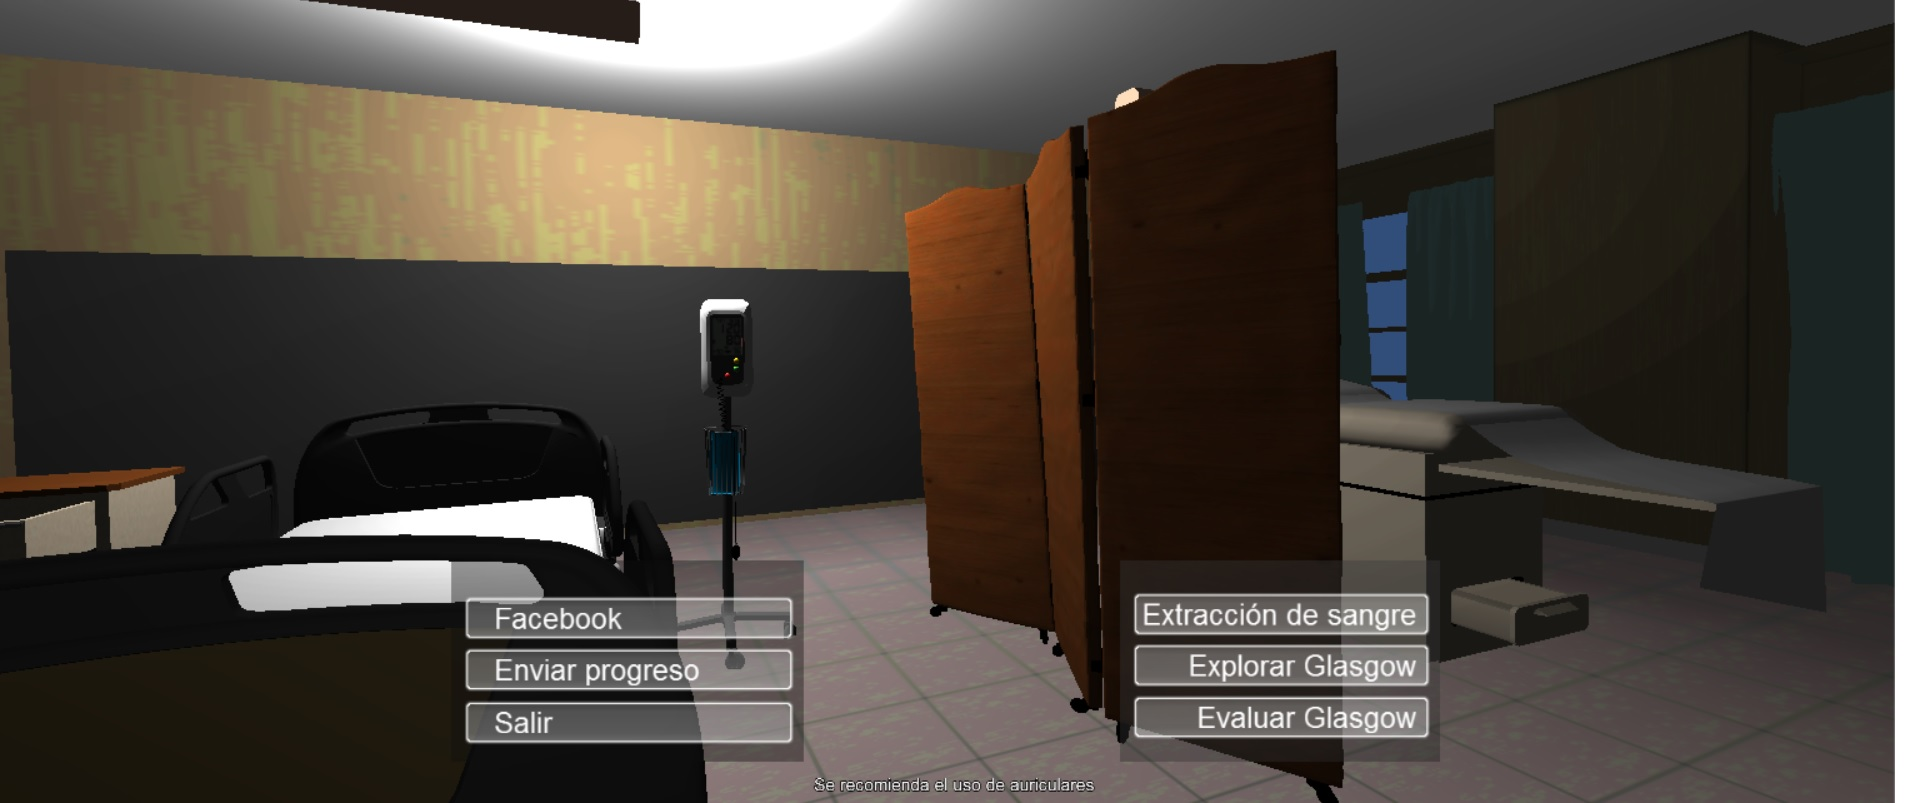
\includegraphics[width=10cm]{solucion/images/pantalla_inicio.jpg}
\caption{Pantalla de inicio de la solución con todas las opciones disponibles.}
\label{fig:pantalla_inicio}
\end{figure}

%\subsubsection{Descripción del entorno}
%\label{sec:inicio_descripcion}


La sala de hospital mostrada como fondo en la figura \ref{fig:pantalla_inicio} es la
que se utiliza como escenografía principal en las escenas de los procedimientos. 
Mientras se muestran las opciones, se ejecuta una animación que recorre el escenario 
mostrando los detalles importantes, como la camilla, el lector de estadísticas vitales, 
y demás elementos del escenario.
%Además de este fondo, se muestran varias opciones en forma de botones que serán
%descriptas a continuación y un mensaje en donde se recomienda al usuario el uso
%de auriculares.

%\begin{figure}[H] 
%\centering 
%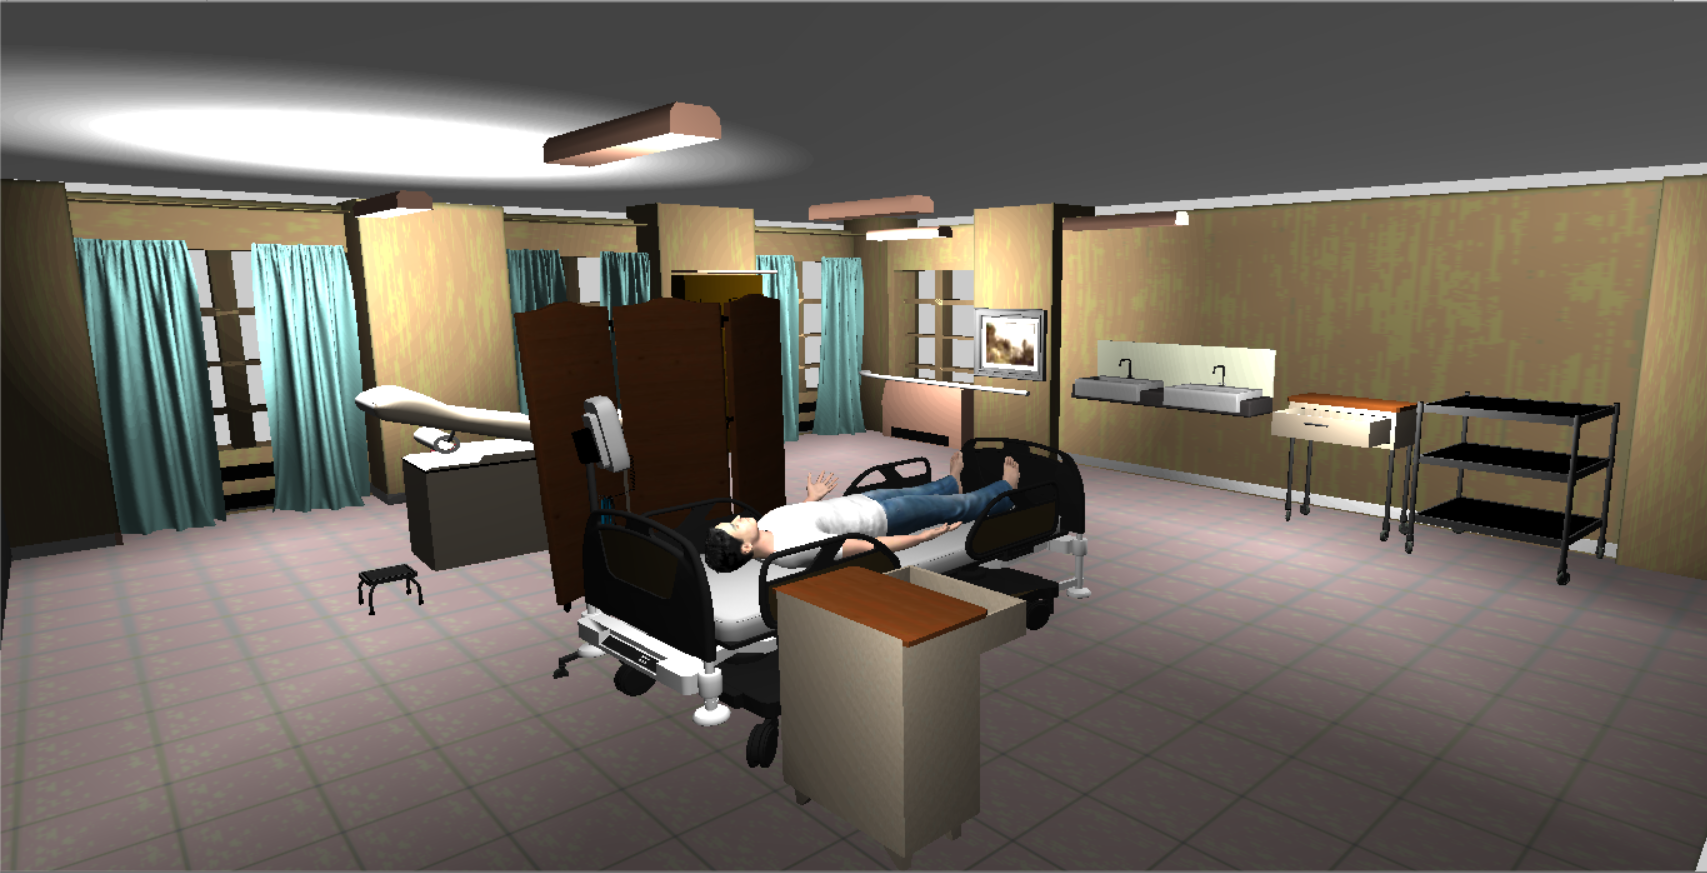
\includegraphics[scale=0.2]{solucion/images/sala.jpg}
%\caption{Edificio y decoración inspirados en los laboratorios de enfermería del
%    \Gls{iab}, este edificio se utiliza para los diferentes escenarios}
%\label{fig:sala_perspectiva}
%\end{figure}


%\observacion{Resumir}

%Se observa en la figura~\ref{fig:pantalla_inicio} la decoración utilizada en
%el escenario \emph{Inicio}, mientras se muestran las opciones, se ejecuta una
%animación que recorre el escenario mostrando los detalles importantes, como la
%camilla, el lector de estadísticas vitales, y demás elementos del escenario.

\subsubsection{Opciones de la pantalla de inicio}

%\observacion{Agregar imágenes con marcos y luego describirlos, en vez de las
    %imágenes actuales con demasiado texto}

%Las opciones disponibles en la pantalla de inicio son presentadas en forma de
%botones los cuales tienen una breve descripción que identifica la función que
%cumplen. 

\begin{itemize}
\item \enquote{Enviar Progreso}: esta función envía toda la información
    acerca de la actividad que el usuario realizó en la aplicación a un servidor
    \emph{backend} que se encarga de almacenar estos datos.
\item \enquote{Salir de la simulación}: esta función permite salir de la
    aplicación.
\item Botón \enquote{Facebook}: esta función permite al usuario ingresar a su
    cuenta de Facebook.
\item \enquote{Extracción de sangre}: esta función permite ingresar a la
    escena correspondiente al procedimiento de extracción de muestras de sangre
    permitiendo al usuario jugar una nueva partida.
\item \enquote{Explorar Glasgow}: esta función permite ingresar a la
    escena correspondiente al procedimiento para explorar las reacción de un
    paciente con un diagnóstico específico de la escala de Glasgow permitiendo
    al usuario jugar una nueva partida.%, el diagnóstico se selecciona una vez
    %presionado este botón a través de la ventana de~\emph{Elegir estado del
    %    paciente}.
\item \enquote{Evaluar Glasgow}: esta función permite ingresar a la escena
    correspondiente al procedimiento para la valoración y diagnóstico de la
    escala de Glasgow para un paciente con estado aleatorio permitiendo al
    usuario jugar una nueva partida.
\end{itemize}


\subsection{Extracción de muestras de sangre}
%\observacion{Agregar pantalla de resultados}

%\observacion{Menos verboso y más imagenes}

Al seleccionar el procedimiento de extracción de sangre en la pantalla de inicio 
la aplicación inmediatamente muestra la escena del procedimiento como se puede 
observar en la figura \ref{fig:hemocultivo_principal}. %, se muestra una 
%sala de hospital igual a la de la pantalla de inicio pero con un paciente en una 
%de las camas, a este paciente es a quien se le realizará el procedimiento.

\begin{figure}[H] 
\centering 
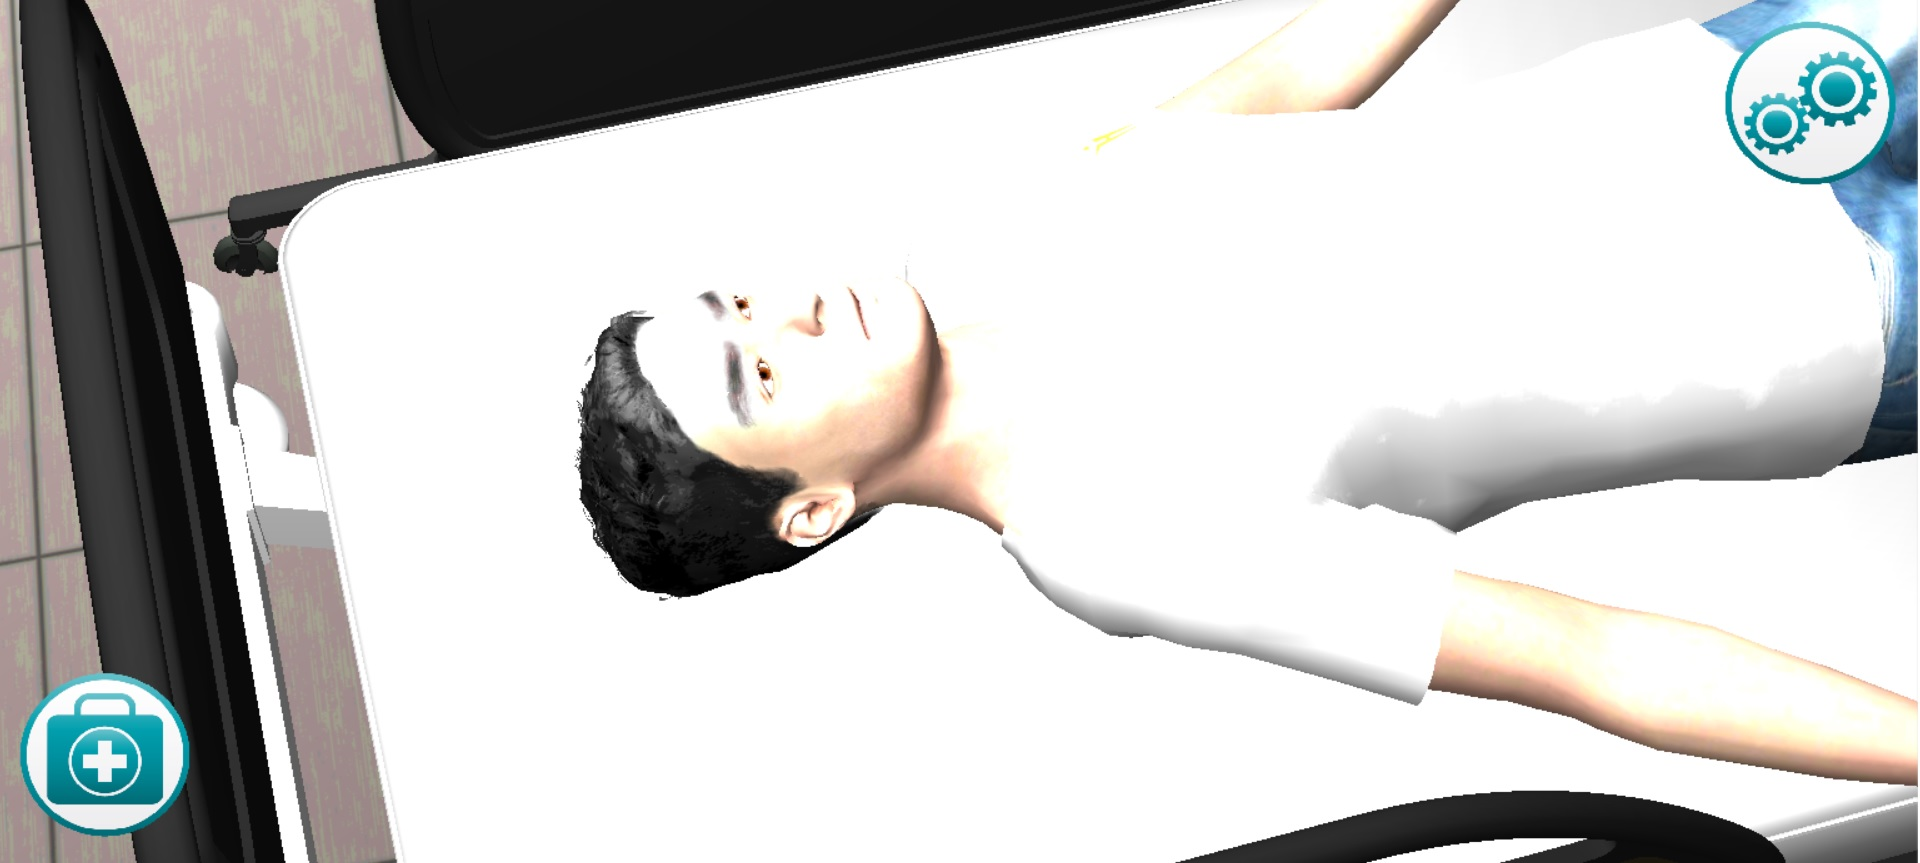
\includegraphics[width=10cm]{solucion/images/hemocultivo_principal.jpg}
\caption{Pantalla principal de la escena del procedimiento de extracción de sangre.}
\label{fig:hemocultivo_principal}
\end{figure}

La posición inicial de la cámara se ubica en un ángulo en donde se puedan ver 
bien los brazos del paciente para facilitar al usuario la realización del 
procedimiento.

A continuación se detallan cada una de las opciones y formas disponibles de
interactuar con la escena del procedimiento de extracción de muestras de sangre.


\subsubsection{Entidades}

En la extracción de sangre existen dos entidades principales, el \emph{paciente}
y el \emph{usuario}, cada entidad mantiene un estado independiente de la otra.
Estas entidades son:

\begin{itemize}

\item \textbf{Paciente:} es una entidad con estado complejo, el cual es
    constantemente modificado por las acciones del usuario, en resumen, la
    información que contiene el paciente es:
    \begin{itemize}
        \item Jeringas\footnote{No se limita la cantidad de jeringas que un
                paciente pueda tener insertadas en un momento dado.}.
        \item Estado de las manos (abiertas o cerradas).
        \item Torniquetes.
        \item Zonas esterilizadas.
        \item Zonas presionadas.
    \end{itemize}

\item \textbf{Usuario:} mantiene un estado en todo momento del cual dependen sus
    acciones, por ejemplo, si la mano del enfermero no está esterilizada,
    cualquier interacción con el paciente provocará que el paciente se
    contamine. La información que contiene la entidad usuario es:

    \begin{itemize}
    \item Estado de las manos.
    \item Estado de la vestimenta (guantes, bata, tapaboca y gorro).
    \item Elemento en uso.
    \end{itemize}
\end{itemize}

\subsubsection{Acciones}

Las acciones que puede realizar el usuario se clasifican en tres, los
\emph{comandos de voz} que simulan una conversación entre el paciente y
enfermero, \emph{las opciones}, que engloban las acciones que puede realizar un
enfermero en cuanto a bioseguridad, y \emph{los elementos} que son las
herramientas que puede utilizar el enfermero durante el procedimiento.

\begin{itemize}
\item{\textbf{Comando de voz}}

Para representar la interacción del usuario con el paciente usando la voz se
implementó un menú que es activado y mostrado en pantalla cuando el usuario
habla, este menú muestra una serie de órdenes que el usuario le diría al
paciente normalmente. Las opciones de menú se detallan a continuación:

\begin{itemize}
    \item \textbf{Explicar procedimiento}: Permite que el usuario explique el
        procedimiento que se va a realizar al paciente. 
\item \textbf{Abrir la mano izquierda}: esta función le indica al paciente que
    abra su mano izquierda, como resultado el paciente realiza esta acción.
\item \textbf{Cerrar la mano izquierda}: esta función le indica al paciente que
    cierre su mano izquierda, como resultado el paciente realiza esta acción.
\item \textbf{Abrir la mano derecha}: esta función le indica al paciente que
    abra su mano derecha, como resultado el paciente realiza esta acción.
\item \textbf{Cerrar la mano derecha}: esta función le indica al paciente que
    cierre su mano derecha, como resultado el paciente realiza esta acción.
\end{itemize}

\begin{figure}[H]
\centering
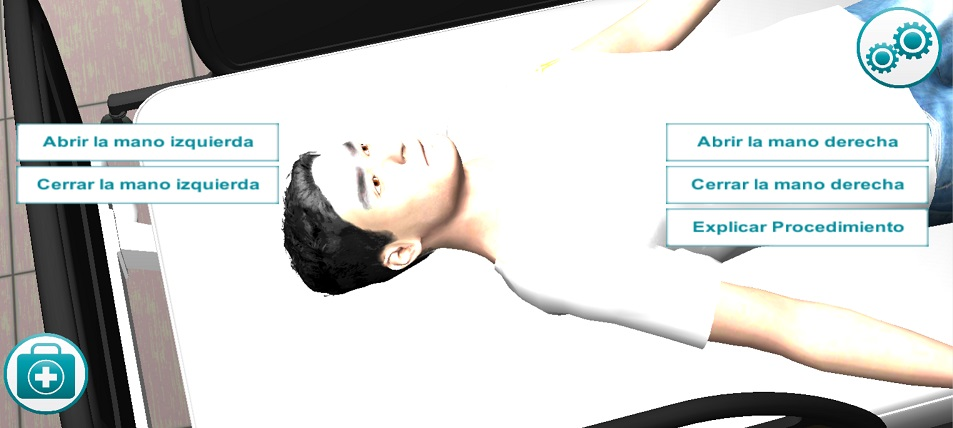
\includegraphics[width=10cm]{solucion/images/hemocultivo_comando_voz.jpg}
\caption{Opciones mostradas al detectar sonido en la escena de extracción
    de sangre.}
\label{fig:hemocultivo_voz_gui}
\end{figure}

En la figura~\ref{fig:hemocultivo_voz_gui} se observan las opciones anteriormente
descritas, este menú aparece inmediatamente después de que el sistema detecte
que el usuario este hablando.

\item{\textbf{Opciones}}

Las \emph{Opciones} son aquellas acciones que puede realizar el usuario y afectan
únicamente al paciente. Representan a los aspectos de bioseguridad, es decir,
acciones como lavarse las manos, calzarse guantes, gorro, bata y tapaboca.

Estas opciones afectan al estado de la entidad \emph{enfermero}.

\item{\textbf{Elementos}}

Los \emph{Elementos} representan las herramientas que utiliza un enfermero
durante el procedimiento, un solo elemento puede ser utilizado en cualquier
momento.


\begin{figure}[H]
\centering
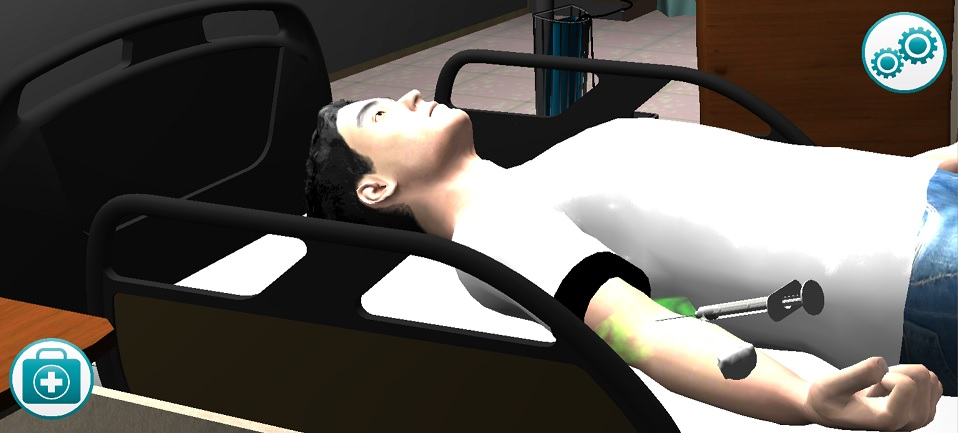
\includegraphics[width=10cm]{solucion/images/hemocultivo_elementos.jpg}
\caption{Interfaz con los elementos en el paciente.}
\label{fig:hemocultivo_elementos}
\end{figure}


Los elementos enumerados en la figura~\ref{fig:hemocultivo_elementos}, son:

\begin{enumerate}
\item \textbf{Torniquete}: es el primer elemento que se debe usar, para
    utilizarlo, se debe presionar una parte del brazo del
    paciente, en ese momento, el torniquete aparece en ese lugar, para
    extraerlo, se debe presionar el torniquete y elegir la opción extraer.

\item \textbf{Esterilizador}: es un elemento que se utiliza para realizar la
    higienización del punto de punción, para utilizarlo se debe presionar
    cualquier parte del brazo del paciente, a continuación aparece una gaza, la
    cual debe ser agitada con un dedo durante un segundo para que se cree una
    zona estéril, la zona estéril creada, es visible a través de una cápsula.

\item \textbf{Jeringa}: Es el elemento utilizado para realizar la extracción, su
    utilización es similar a la del \emph{Torniquete}.

    A través de un menú contextual, se ofrece la posibilidad de realizar un
    acercamiento, como se observa en la figura~\ref{fig:hemocultivo_jeringa_zoom}, 
    en la vista ampliada, se puede realizar la extracción de sangre utilizando dos dedos, 
    con el primero se presiona el tambor y con el segundo dedo se extrae el émbolo\footnote{El
    tambor es la parte de la jeringa que almacena el fluido, mientras que el
    émbolo es la parte que se utiliza para presionar o succionar el fluido}.
    
\item \textbf{Algodón}: El algodón se utiliza para presionar una zona que
    recientemente fue punzada, para utilizar este elemento, basta con presionar
    el brazo del paciente durante un segundo.

\end{enumerate}


\begin{figure}[H]
\centering 
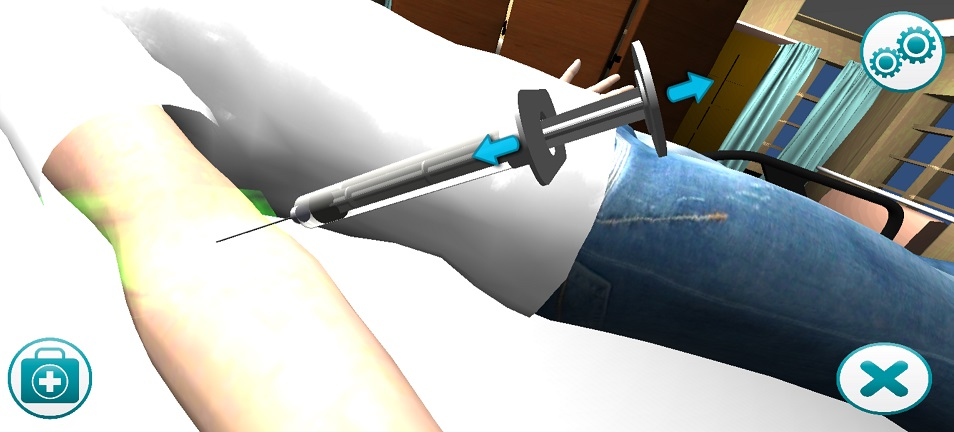
\includegraphics[width=10cm]{solucion/images/hemocultivo_jeringa_ampliada.jpg}
\caption{Vista de la jeringa ampliada, facilitando la extracción de sangre. Se
    agregan flechas azules para facilitar la comprensión del cómo se extrae
    sangre.}
\label{fig:hemocultivo_jeringa_zoom}
\end{figure}

\end{itemize}

\subsubsection{Reglas para la evaluación durante la ejecución}

%\observacion{Si hay orden tienen que enumerar}
%\observacion{Quizás haya una manera de visualizar esto, para que se vea el orden
    %y las dependencias}
%\observacion{Definitivamente hay que visualizar esto y reducir la descripción
    %total. En todo caso hacer comentarios sobre cosas demasiado importantes
    %después, pero una lista como seta es demasiada sobreiformación y no se
    %entiende}


Las reglas definidas dentro de la extracción de sangre definen las acciones
que se deben llevar a cabo para completar el procedimiento, es necesario que
todas las reglas sean cumplidas para obtener un puntaje perfecto.

Cada regla contiene información acerca del estado del progreso del alumno en un
paso en particular, estas reglas pueden tener como dependencias a otras reglas,
es decir, una regla sólo se puede cumplir si una regla anterior se cumple, este
es el caso de las reglas que definen la extracción de un torniquete, la cual
depende de la regla que define la colocación del torniquete.  

Las reglas definen el mecanismo que se utiliza para proveer una retroalimentación
al usuario una vez finalizada la partida, pues almacena información 
acerca del progreso del usuario en cada paso.

A continuación se muestran cada una de estas reglas en la
tabla~\ref{tab:reglas_hemocultivo}, en donde se detallan cada uno de los estados
por los que pasa, a excepción de los estados BEGIN y FINISH que sólo indican el
inicio y fin de una regla. Una regla se cumple si se cumplen todas las reglas de
las cuales depende, si se lanzan los eventos esperados y si la condición del
entorno es la esperada.


\begin{table}[H]
\centering
\begin{tabulary}{\textwidth}{LLRRR}
\toprule
& Regla & Depende de las reglas & Espera a los eventos & Cuando se cumple que \\
\midrule
1  & Explicar procedimiento    &         & Explicar procedimiento    & Sea la primera regla lanzada\\
2  & Higienización de manos    & 1       & Higienización de manos    &\\
3  & Ponerse tababoca          & 2       & Ponerse tababoca          & Se realize antes de ponerse los guantes\\
4  & Ponerse gorro             & 2       & Ponerse gorro             & Se realize antes de ponerse los guantes\\
5  & Ponerse bata              & 2       & Ponerse bata              & Se realize antes de ponerse los guantes\\
6  & Calzar guantes            & 2,3,4,5 & Calzar guantes            &\\
7  & Colocar torniquete        & 10      & Colocar torniquete        & La zona correcta y mismo brazo de inserción\\
8  & Cerrar manos              & 7,10    & Cerrar puño               & Sea el mismo brazo que inserción\\
9  & Esterilizar zona          & 10      & Esterilizar zona          & Sea la misma zona que inserción\\
10 & Realizar punción          & 2       & Realizar punción          & Sea la zona correcta\\
11 & Retirar Torniquete        & 10,7    & Retirar Torniquete        & Sea el mismo torniquete que activo regla 7\\
12 & Abrir mano                & 10,8    & Abrir mano                & Sea la misma mano que activo regla 8\\
13 & Extraer Sangre            & 10,12   & Extraer Sangre            &\\
14 & Retirar Jeringa           & 10      & Retirar Jeringa           & Sea la misma jeringa que activo regla 10\\
15 & Presionar zona de punción & 10      & Presionar zona de punción & Sea la misma zona de punción\\
16 & Quitar tapaboca           & 10,3    & Quitar tapaboca           &\\
17 & Quitar gorro              & 10,4    & Quitar gorro              &\\
18 & Quitar bata               & 10,5    & Quitar bata               &\\
19 & Descalzar guantes         & 10,6    & Descalzar guantes         &\\
20 & Limpiar manos             & 19      & Limpiar manos             &\\
\bottomrule
\end{tabulary}
\caption{Reglas definidas para el procedimiento de extracción de sangre, se muestran los detalles de cada uno 
de los estados por los que pasan cada una de las reglas.}
\label{tab:reglas_hemocultivo}
\end{table}
%La reglas del procedimiento de extracción de sangre fueron definidas de acuerdo
%a los pasos requeridos según el protocolo del procedimiento y al orden en el que
%son requeridos. Es decir, cada paso del protocolo tiene asociado una regla
%dentro del motor que lo representa y las condiciones asociadas a cada regla
%están determinadas por el orden en que deben realizarse dentro del protocolo.

%Cada regla tiene una o mas condiciones que deben ser cumplidas para que un paso
%del protocolo realizado se considere correcto.


%\begin{itemize}
%\item \textbf{Explicar procedimiento}: define cuando el usuario ha explicado el
%    procedimiento, debe ser la primera regla que se cumple, existiendo dos
%    estados que no cumplen la condición, cuando no es la primera regla que se
%    cumple y cuando el usuario no realizó la acción.

%\item \textbf{Higienización de manos}: define sí las manos del enfemero están
%    limpias, existen dos estados para esta regla, cuando se lavó las manos y
%    cuando no realizó esta acción. Es importante notar que de esta regla
%    dependen varias reglas posteriores, es decir, si esta regla no se cumple,
%    las reglas de bioseguridad no pueden ser cumplidas.

%\item \textbf{Calzar guantes}: este paso es inmediatamente posterior a la
%    higienización de las manos, y como este, varias reglas dependen del momento
%    en el que se calcen los guantes. Si el paciente se calza los guantes, la
%    única forma de equivocarse en este paso es que las manos estén sucias.

%\item \textbf{Gorro, bata y tapaboca}: estos tres pasos son similares, pues
%    tienen las mismas dependencias y el orden en el que se cumplan no está
%    definido, las posibilidades con este paso son:
%    \begin{itemize}
%    \item Incompleto: si el usuario no se puso el gorro, bata o tapaboca en
%        ningún momento de la práctica.
%    \item Manos sucias: si la regla \emph{Higienización de manos} no se cumple
%        cuando el usuario se vista con el gorro, bata o tapaboca.
%    \item Sin guantes: si la regla \emph{Calzar guantes} no se cumple al momento
%        de ponerse el gorro, tapaboca o bata. 
%    \end{itemize}
    
%\item \textbf{Colocar torniquete}: este paso debe ser realizado una vez que el
%    usuario tenga el guante calzado, el torniquete puede ser colocado en
%    cualquier parte del brazo, pero depende del lugar de punción de la jeringa.
%    Así, existen dos casos donde esta regla falla, cuando no se coloca el
%    torniquete en ningún lugar, y cuando el torniquete se coloca en un lugar
%    inadecuado. Es importante notar que esta regla se activa cuando se realiza
%    la punción de la jeringa.

%\item \textbf{Cerrar manos}: debe ocurrir después de que se explique el
%    procedimiento y antes de que se inserte la jeringa, además deberá ser la
%    mano correspondiente al lugar donde se inyectó la jeringa. Así, existen dos
%    formas de no realizar correctamente este paso, que la punción haya ocurrido en otro brazo, o
%    que la punción no se realizó. Es importante notar que esta regla no se activa
%    cuando el usuario solicita al paciente que cierre su mano, sino cuando la
%    jeringa es insertada, esto es así pues es importante el estado de la mano
%    cuando el usuario realiza la punción.

%\item \textbf{Esterilizar zona}: El usuario puede esterilizar varias zonas, pero
%    la única zona que activa esta regla, es aquella donde se realizó la punción.
%    Así esta regla tiene dos posibles formas de proveer retroalimentación en
%    caso de que no se cumpla, que no se esterilizó ningún lugar del cuerpo, o
%    que el lugar esterilizado no sea el lugar de punción.

%\item \textbf{Realizar punción}: Existen dos casos de error, si el usuario
%    inserta la jeringa en un lugar incorrecto (los lugares correctos se definen
%    en~\ref{sec:hemocultivo_hipotesis}), y si el usuario no realiza la punción.

%\item \textbf{Retirar Torniquete}: esta regla es dependiente de la regla
%    \emph{Colocar Torniquete}, y de qué torniquete se retira. Existiendo dos
%    casos de error, el usuario retira un torniquete que no activó la regla
%    \emph{Colocar Torniquete} (indicando que este es el torniquete correcto), y
%    que no se retire ningún torniquete.

%\item \textbf{Abrir mano}: una vez realizada la punción, y retirado el torniquete,
%    se debe solicitar al paciente que abra sus manos, así, es dependiente de la
%    regla \emph{Realizar punción}, y tiene tres casos de error, que la punción
%    no se haya realizado, que la mano no se haya cerrado antes, y que la mano
%    que se abra no corresponda con la mano que se cerró.

%\item \textbf{Extraer Sangre}: depende únicamente de si la jeringa con la cual
%    se extrae sangre es la correcta, así hay dos posibles casos de error, que
%    la sangre no se haya extraído, y que la regla \emph{Realizar punción} no se
%    cumpla.

%\item \textbf{Retirar Jeringa}: se controla que la jeringa que se extraiga sea
%    la jeringa que cumplió el paso \emph{Realizar punción}, así, existen dos
%    casos de error, que la jeringa no hay sido extraída y que se extrajo sangre
%    de una jeringa incorrecta.

%\item \textbf{Presionar zona de punción}: debe realizarse inmediatamente después
%    de \emph{Retirar Jeringa}, y tiene dos casos de error, que la jeringa no
%    haya sido extraída, y que la zona presionada no corresponda con la zona de
%    punción.

%    \item \textbf{Quitar bata, gorro y tapaboca}: depende de la regla \emph{Bata,
%        gorro y tapaboca}, y de que la jeringa haya sido extraída, si el
%    enfermero se extrae la bata, gorro o tapaboca antes de retirar la jeringa, se
%    produce un error. Otro caso para que esta regla no se cumpla es que la regla
%    \emph{Bata, gorro y tapaboca} no se cumpla.

%\item \textbf{Descalzar guantes}: depende de que las reglas \emph{Calzar
%        Guantes} y \emph{Retirar jeringa}, así existen dos posibles casos de
%    error, que el usuario no se calce los guantes, o que la jeringa no haya sido
%    extraída.

%\item \textbf{Limpiar manos}: Como paso final, se debe proceder a realizar una
%    higienización de manos, este debe ser el paso final, y tiene como
%    prerrequisito que todas las reglas anteriores hayan sido lanzadas.

%\end{itemize}

%\subsection{Pantalla de resultados}

\subsubsection{Retroalimentación y puntuación final}
\label{sec:puntuacion_hemocultivo}

Al final de una partida, la solución le brinda una retroalimentación al 
usuario como se muestra en la figura~\ref{fig:hemocultivo_retroalimentacion}.

\begin{figure}[H]
\centering 
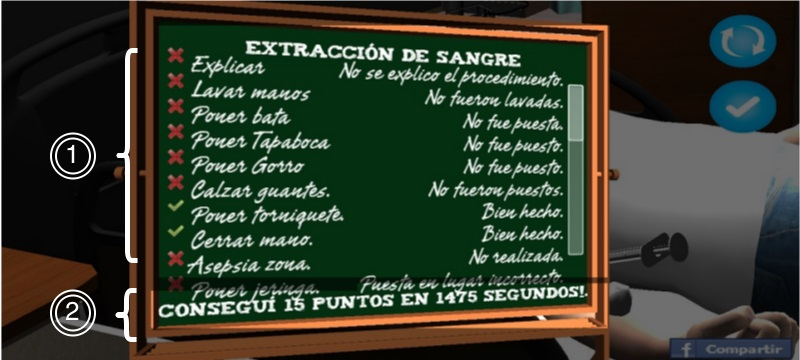
\includegraphics[width=10cm]{solucion/images/hemocultivo_retroalimentacion.jpg}
\caption{Retroalimentación y puntuación final del procedimiento de extracción de sangre.}
\label{fig:hemocultivo_retroalimentacion}
\end{figure}

En la parte $1$ de la figura~\ref{fig:hemocultivo_retroalimentacion} , se puede ver 
como se brinda información al  usuario acerca de su rendimiento. Esta información le 
indica los pasos que realizó de manera correcta o incorrecta y las razones por las 
cuales tuvo ese desempeño.

Como se describió anteriormente, una regla puede quedar en uno de diferentes
estados al final de la partida, cada uno de esos estados posee un significado en
el contexto del procedimiento y por lo tanto tienen información asociada para
brindar información al final de la partida.

Cada regla tiene asociado un peso, de acuerdo a la dificultad de realizar el
paso, este peso es utilizado al final de la partida para darle una puntuación al
usuario como se muestra en el punto $2$ de la
figura~\ref{fig:hemocultivo_retroalimentacion}. Junto al puntaje final también
se muestra el tiempo que le tomó al usuario completar el procedimiento.


\subsubsection{Registro de actividad}

%El registro de actividades del usuario dentro de la solución es utilizado ya 
%que es necesario una evaluación posterior del rendimiento de la solución así como 
%su uso e impacto en el usuario.

%La información que se almacena permite reproducir exactamente todo el desarrollo
%de la simulación, con excepción de los movimientos de la cámara. De esta manera,
%los datos recabados permiten saber en que tareas los usuarios se encontraron con
%un mayor número de inconvenientes.

Cada acción que realiza el usuario dentro de la simulación provoca un evento, y
estos eventos son registrados de manera transparente para el usuario. Como así 
también los eventos que genera la aplicación y el motor de reglas.

Existen otros tipos de eventos que no son generados por acciones, por ejemplo,
cuando la simulación termina, el motor de reglas lanza un evento por regla,
indicando su estado.

El registro de actividades permite reproducir las partidas y por lo tanto, es 
posible determinar que tareas fueron con las que los usuarios tuvieron un 
mayor número de inconvenientes.

%Un subconjunto de todos los eventos, son registrados en un archivo de texto en
%formato \Gls{json}, el mismo es posteriormente enviado a un servidor que
%almacena la información de todos los usuarios.

El registro de actividades se almacena en el dispositivo del usuario, y luego
es enviado al \emph{backend}, esto se explica con más detalle
en~\ref{sec:backend_reg_eventos}. En la tabla \ref{tab:hemocultivo_registro} 
se pueden observar los eventos registrados.

%Los eventos registrados, son aquellos que involucran a las opciones, elementos,
%utilización de la jeringa, torniquete, higienización, y como un caso especial,
%todas las reglas también son registradas (independientemente de si son
%satisfactorias o no).


\begin{table}[H]
\centering
\begin{tabulary}{\textwidth}{|L|L|L|}
\hline
Acción & Eventos & Motivos \\
\hline
Preparación del paciente & Explicación del procedimiento & Validación de interfaz intuitiva, 
de realización correcta de pasos y de la hipótesis \enquote{Comandos de voz} \\
\hline
Bioseguridad inicial  & Lavado de manos, calzado de guantes, bata, tababoca y gorro & Validación 
de interfaz intuitiva, de realización correcta de los pasos y de la hipótesis 
\enquote{Opciones de Bioseguridad} \\
\hline
Preparación para la extracción & Esterilización de zona, colocación de torniquete, petición de cierre de mano 
& Validación de interfaz intuitiva, de realización correcta de pasos y de validación de la hipótesis \enquote{Comandos de voz} \\
\hline
Punción y extracción & Punzado, extracción de torniquete, petición de apertura de mano, extracción de sangre, 
extracción de jeringa & Validación de interfaz intuitiva, de realización correcta de pasos y de la 
hipótesis \enquote{Comandos de voz} \\
\hline
Post - extracción & Presionar zona de punción & Interfaz intuitiva, realización correcta del paso \\
\hline
Bioseguridad final & Lavado de manos, descalzado de guantes, bata, tapaboca y gorro & Validación de interfaz intuitiva, de realización correcta de los pasos y de la hipótesis \enquote{Opciones de Bioseguridad} \\
\hline
Utilización de redes sociales & Socialización del resultado de la partida & Medición del efecto motivador\\
\hline
\end{tabulary}
\caption{Acciones registradas durante una partida del procedimiento de extracción de sangre, los eventos 
relacionados a ellas, y los motivos de sus registros.}
\label{tab:hemocultivo_registro}
\end{table}



\subsubsection{Interfaz del usuario}

La interfaz principal de este escenario posee dos menús como se indica en la figura 
\ref{fig:hemocultivo_gui} con los números $1$ y $2$, las opciones dentro cada menú poseen 
una imagen intuitiva que representa la función que realizan. Al menú número uno lo llamaremos 
\emph{Elementos} y al número dos \emph{Opciones}.

\begin{figure}[H]
\centering
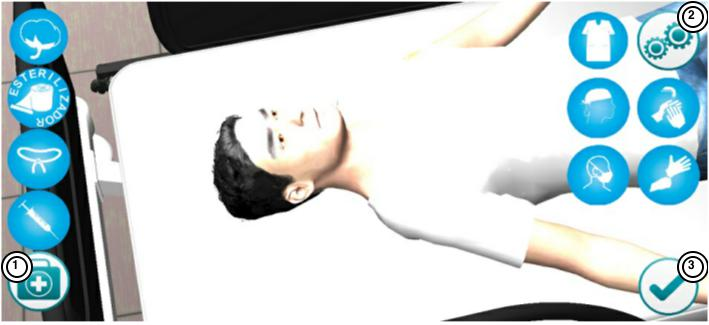
\includegraphics[width=10cm]{solucion/images/hemocultivo_menus.jpg}
\caption{Vista de la interfaz principal del escenario \emph{Extracción de
        sangre}, con todas las opciones desplegadas.}
\label{fig:hemocultivo_gui}
\end{figure}


%En la figura~\ref{fig:hemocultivo_gui} se observa la interfaz, se muestra en el
%centro al paciente, y las diferentes opciones que tiene el usuario para
%interactuar con el paciente y consigo mismo como enfermero.

%Existen dos opciones principales dentro de la interfaz, en la parte superior
%derecha se encuentra el menú \emph{Opciones} y en la parte superior izquierda, el menú
%\emph{Elementos}.

Al presionar el menú \emph{Opciones} aparecen las distintas
acciones que puede realizar el usuario en cuanto a aspectos de bioseguridad, 
todos los botones afectan al estado del usuario o enfermero. Con excepción 
del lavado de manos, las opciones disponibles representan el hecho de 
ponerse/sacarse los guantes, el tapaboca, el gorro y la bata, esto se da 
seleccionando/deseleccionando estas opciones. Además se brinda la opción de 
finalizar la partida con el botón indicado con el número $3$.

%el
%lavado de manos es idempotente, \fixme{es decir no importa cuantas veces se
%    presione, el resultado será el mismo, en cambio los demás botones (bata,
%    guante, tapaboca y gorro) representan la acción de calzar}{Hace falta tanto
%    detalle?}/descalzar, es decir, la primera vez que se presiona la opción
%bata, el estado del enfermero cambia a \emph{Con Bata}, si se presiona una
%segunda vez, el estado cambia a \emph{Sin Bata}.

En el menú \emph{Elementos} se despliegan opciones que representan a lo elementos que se
utilizan para realizar el procedimiento, una vez presionado un elemento queda
seleccionado (simulando que es la herramienta que el enfermero tiene en la mano
en ese momento), sólo un elemento puede ser seleccionado a la vez. Si el mismo
botón se vuelve a presionar inmediatamente después de haber sido presionado, el
elemento se des-selecciona (simulando que el enfermero dejó la herramienta).


Adicionalmente, existen dos tipos de indicadores mostrados en la figura
\ref{fig:hemocultivo_seleccion}. El tipo de indicador marcado con el $1$l
representa el elemento actualmente seleccionado y el tipo de indicador marcado
con el $2$ representan al estado actual del usuario o enfermero en cuanto a
aspectos de bioseguridad referentes a vestimentas de protección personal.
%Adicionalmente, existen dos indicadores del estado del paciente, en la parte
%inferior derecha, denominados \emph{Indicadores de bioseguridad}, se muestran
%iconos representando los elementos que tiene actualmente el enfermero, estos
%incluyen los gorros, bata y tapaboca. El elemento que actualmente esta
%seleccionado se muestra en la parte superior izquierda de la pantalla, a
%diferencia de los indicadores de bioseguridad, se muestra un único icono a la vez.

\begin{figure}[H]
\centering
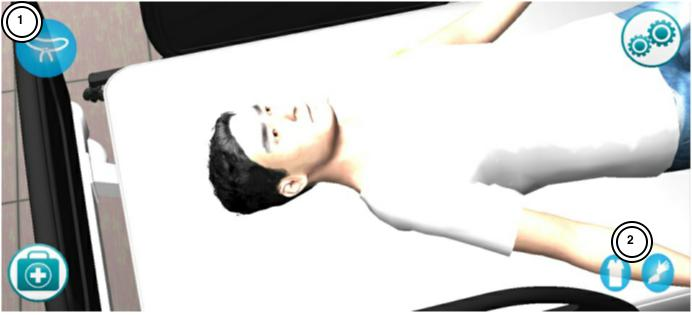
\includegraphics[width=10cm]{solucion/images/hemocultivo_seleccion.jpg}
\caption{Indicadores de selección de elementos y de estado de usuario o enfermero.}
\label{fig:hemocultivo_seleccion}
\end{figure}



Por último, para la utilización de los elementos, existe un menú contextual\footnote{Un menú
    que se despliega al presionar un elemento, es contextual pues varía de
    acuerdo al elemento seleccionado.}, que lista las opciones disponibles por
elemento, como se observa en la figura~\ref{fig:hemocultivo_torniquete_cm}.

\begin{figure}[H]
\centering
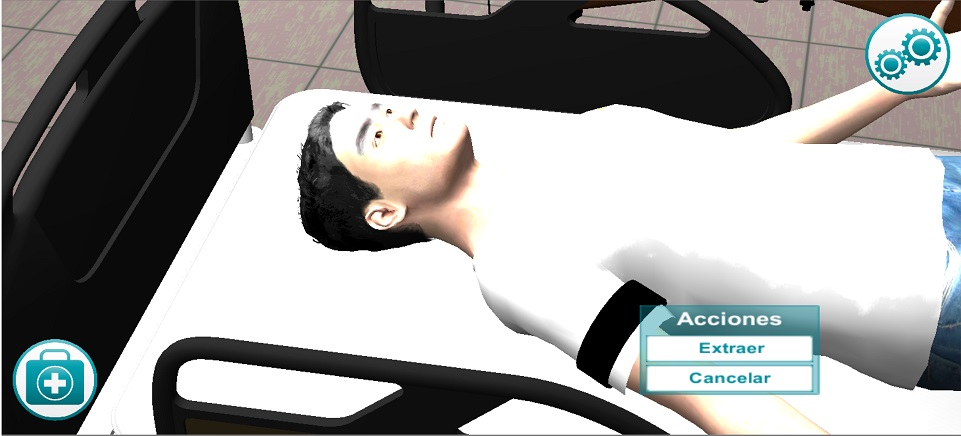
\includegraphics[width=10cm]{solucion/images/hemocultivo_contextual.jpg}
\caption{Menú contextual del elemento torniquete.}
\label{fig:hemocultivo_torniquete_cm}
\end{figure}

\subsection{Valoración de la escala de Glasgow}

La escena  \emph{Valoración de la escala de Glasgow} %busca simular el
%comportamiento de un paciente con daño cerebral, por ello 
se presenta en dos
modos distintos, en el primero, el usuario no conoce el estado del paciente,
este modo se conoce como \emph{Evaluar Glasgow}, y en su segundo modo, el
usuario elige el estado del paciente antes de iniciar la escena, esto modo
se conoce como \emph{Exploración Glasgow}. 

La reducida cantidad de diferencias entre ambos modos de la práctica permiten
que ambas sean descritas en esta sección, las características explicadas son
comunes para ambas, salvo que se especifique lo contrario.

En el modo \emph{Exploración Glasgow}, antes de iniciar la práctica, se le
permite al usuario seleccionar el estado del paciente mediante una interfaz 
como se puede observar en la figura \ref{fig:glasgow_seleccion}, en
cambio, en el modo \emph{Evaluar Glasgow}, el estado del paciente no se conoce
de antemano y será responsabilidad del usuario determinarlo.

\begin{figure}[H]
\centering
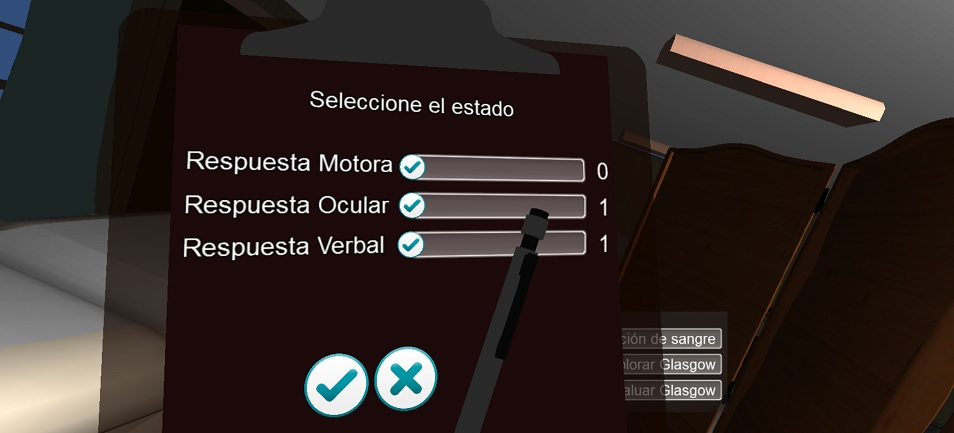
\includegraphics[width=10cm]{solucion/images/glasgow_seleccion.jpg}
\caption{Interfaz del modo \emph{Exploración Glasgow} para seleccionar el estado del 
paciente.}
\label{fig:glasgow_seleccion}
\end{figure}

La pantalla principal de este procedimientos es como se muestra en la figura
\ref{fig:glasgow_principal}, en ella además del paciente sólo se ofrece una
opción para finalizar la partida actual.

\begin{figure}[H]
\centering
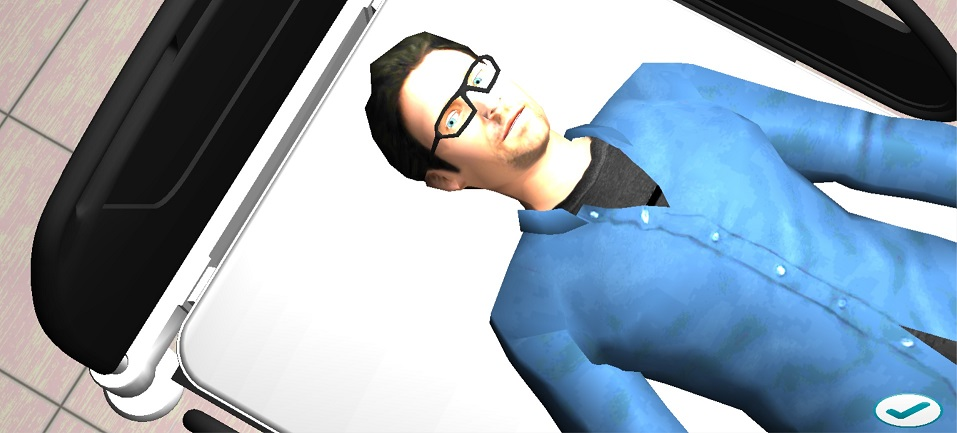
\includegraphics[width=10cm]{solucion/images/glasgow_principal.jpg}
\caption{Pantalla principal de la escena de valoración de la escala de Glasgow.}
\label{fig:glasgow_principal}
\end{figure}

%Existe una pantalla particular dentro de esta escena, conocida como
%\emph{Pantalla de Diagnóstico}, esta pantalla, permite al usuario ingresar su
%diagnóstico del paciente, contiene cuatro preguntas básicas, la valoración
%motora, verbal, ocular y general de acuerdo a lo definido en~\ref{sec:glasgow} y
%a las hipótesis definidas en~\ref{sec:glasgow_hipotesis}.

\emph{Exploración Glasgow}.

\subsubsection{Entidades}

Existen dos entidades principales, el usuario o \emph{Enfermero} y el \emph{Paciente}, 
el enfermero no almacena información, y el
paciente sólo almacena su estado, que se define al inicio. De esta forma, las
entidades no se modifican en ningún momento.

La información almacenada por la entidad paciente es su estado motor, verbal y
ocular, el cual es un conjunto de números, cuyos posibles valores se definen en
en~\ref{sec:glasgow_protocolo}, la definición de estos números varían de acuerdo
al tipo de la escena:

\begin{itemize}
    \item \textbf{Exploración}: donde el usuario selecciona el estado
        del paciente que desea, este estado se mantendrá constante durante toda
        la escena.
    \item \textbf{Evaluación}: al inicio se crean tres números de manera
        aleatoria, el algoritmo que crea estos valores, lo hace de tal manera
        que el estado del paciente es consistente, por ejemplo, el paciente
        nunca tendrá un estado verbal \enquote{Orientado} (valor 5 en la escala)
        y un estado ocular \enquote{Ausente} (valor 1 en la escala), pues esto
        no tendría sentido, si no puede abrir los ojos (estado
        \enquote{ausente}), no puede saber donde esta (estado
        \enquote{orientado}).
\end{itemize}

Aunque el estado de las entidades no se modifique, esto no significa que no
puedan realizar acciones entre ellas, sino que estas acciones y los eventos
generados no alteran el estado de las entidades.

\subsubsection{Acciones} 

Las acciones se clasifican en dos tipos, los \enquote{comandos de voz} y las
\enquote{opciones a través de menú contextual}. 

\begin{itemize}
\item{\textbf{Menú Contextual}}

Las opciones a través del menú contextual se relacionan a acciones que puede
realizar el enfermero sobre una parte particular del cuerpo del paciente, en las
extremidades, el menú despliega una sola opción, la cual es \emph{Pinchar}, que
provoca que el enfermero realice un estímulo doloroso al paciente, el
paciente reacciona ante este estímulo dependiendo de su valoración motora y
ocular. 

\begin{itemize}
    \item Si el estado ocular del paciente es \enquote{Al dolor}, el paciente
        abrirá los ojos inmediatamente después de que se presione la opción. 
    \item  La respuesta motora varía de acuerdo a su estado, si el mismo es
        \enquote{Localiza}, el paciente mueve sus manos hasta el origen del
        dolor, si el estado es \enquote{Retira}, moverá la extremidad que
        sufrió el estímulo lejos de su posición inicial, si es
        \enquote{Flexión anormal}, el paciente reaccionará comprimiendo el
        cuerpo, indistintamente de la ubicación del estímulo doloroso, y si el
        estado es \enquote{Extiende}, el paciente extenderá el cuerpo también 
        indistintamente de la ubicación del estímulo doloroso.
\end{itemize}

\item{\textbf{Comandos de voz}}

Las opciones disponibles a través de los comandos de voz, simulan una
interacción verbal entre el enfermero y el paciente, y se agrupan en tres
tipos, verbales, oculares y motoras.

Las preguntas y posibles respuestas de tipo \emph{verbal}, se pueden ver en la
tabla~\ref{tab:glasgow_opciones_respuesta}. 

\begin{table}[H]
\centering
\begin{tabulary}{\textwidth}{LCCCCC}
\toprule
\textbf{Pregunta} & \textbf{Orientado} & \textbf{Confusa} & \textbf{Palabras
    inapropiadas} & \textbf{Palabras incomprensibles} & \textbf{Ausente} \\
\midrule
¿Qué día es? & El día de la semana actual & Cualquier día de la semana menos el
correcto & La respuesta a otra pregunta en estado orientado & Gritos, gruñidos y
quejidos & No emite sonido \\
¿Cuál es su nombre? & \emph{Carlos Benitez} & Respuesta coherente sin mencionar
su nombre & Respuesta a otra pregunta en estado orientado & Gritos, gruñidos y
quejidos & No emite sonido \\
¿Donde se encuentra? & \emph{En una cama de hospital} & \emph{En mi dormitorio} &
Respuesta a otra pregunta en estado orientado & Gritos, gruñidos y quejidos & No
emite sonido \\
\bottomrule
\end{tabulary}
\caption{Posibles respuestas de acuerdo al estado verbal del paciente.}
\label{tab:glasgow_opciones_respuesta}
\end{table}

Las opciones del menú por comandos de voz del tipo \emph{motor}, son cuatro: 

\begin{itemize*}
    \item Mueva el brazo
    \item Mueva la pierna
    \item Mueva la mano
    \item Mueva la cabeza
\end{itemize*}

Estas opciones no tienen una respuesta sonora, en cambio, si el estado motor es
\enquote{Obedece},el paciente reacciona moviendo una extremidad, en caso
contrario, el paciente no realiza acción alguna.

Finalmente, existe una opción \emph{ocular}, la cual es \enquote{Abra sus ojos por
favor}, la cual no tiene una respuesta sonora, y sólo si el paciente tiene un
estado ocular \enquote{Al hablar} abre los ojos, en caso contrario, no realiza
acción alguna.

\end{itemize}

\subsubsection{Evaluación}
\label{sec:puntuacion_glasgow}

La evaluación del desempeño del usuario en la partida sólo se da en el modo \emph{Evaluación 
Glasgow}. A continuación se describe la el método de evaluación del procedimiento 
de valoración de la escala  de Glasgow, se empieza describiendo como el 
usuario registra su valoración en la solución.

\begin{itemize}
\item{\textbf{Pantalla de diagnóstico}}

Una vez que el usuario decida que está listo para dar un diagnóstico, procede a
finalizar la escena, en ese momento se presenta una pantalla donde el mismo
puede diagnosticar al paciente, como se observa en la
figura~\ref{fig:glasgow_gui_resultados}.

Las opciones presentadas al usuario son cuatro, puntuación verbal, ocular,
motora y un diagnóstico del estado de conciencia del paciente. Estos valores
se describen en~\ref{sec:glasgow_protocolo}.

\begin{figure}[H]
\centering
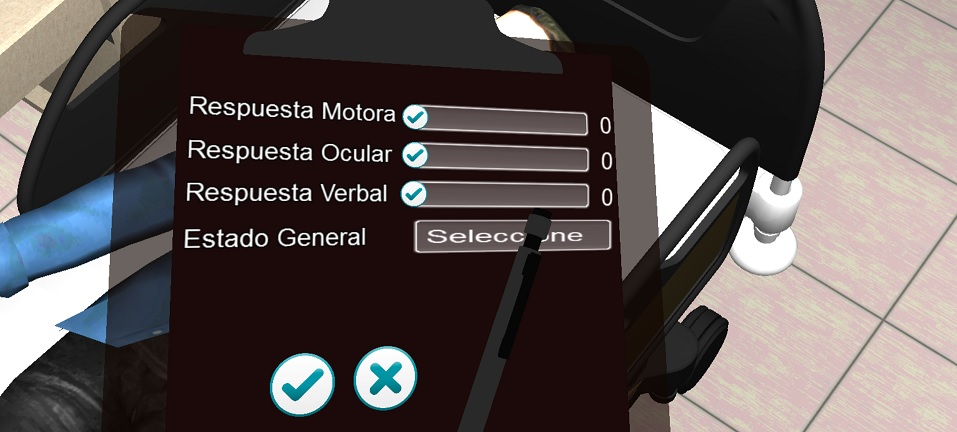
\includegraphics[width=10cm]{solucion/images/glasgow_diagnostico.jpg}
\caption{Vista de la \emph{Pantalla de diagnóstico}, donde el usuario puede
    asignar una puntuación a cada aspecto analizado del paciente.}
\label{fig:glasgow_gui_resultados}
\end{figure}

%En el modo \emph{Evaluación Glasgow}, esta misma pantalla se utiliza la inicio
%de la escena para que el usuario pueda seleccionar el estado deseado del
%paciente.

%La única diferencia que existe entre la \emph{Pantalla de diagnóstico} entre la
%exploración y la evaluación, es que en la evaluación, los posibles valores para
%cada aspecto a diagnosticar van de $0$ a $8$, y en la exploración, son los
%valores mínimos y máximos válidos\footnote{Los valores máximos se definen
%    en~\ref{sec:glasgow_protocolo} y son $4$ (ocular), $5$ (verbal) y $6$
%    (motora)}.


\item{\textbf{Retroalimentación y puntuación final}}

%Como se explicó en el capítulo \ref{chap:requerimientos}, un paciente puede estar 
%en ciertos estados específicos dentro de la escala, y además dentro de cada estado 
%reacciona de una forma en particular, por lo tanto, al inicio de la partida un 
%componente interno de la aplicación selecciona de forma aleatoria un estado para 
%el paciente, de forma tal que cada vez que una partida sea jugada no se repitan 
%los estados de forma seguida.

El estado aleatorio del paciente que es generado al inicio de la partida 
es guardado en una variable que no es modificada hasta que se reinicie la partida. 
Al final de la partida, la aplicación pide al usuario que valore el estado del paciente 
que le fue presentado, una vez que el usuario confirme su respuesta la aplicación la
compara con el estado guardado y de esta forma puede informar al usuario acerca
de su rendimiento en el diagnóstico. 

Además, cada posible respuesta dada por el usuario contiene información
relacionada al contexto del procedimiento y a la situación actual presentada, la
cual, es utilizada como retroalimentación al final de la partida como puede verse 
en la figura \ref{fig:glasgow_resultado} marcado por el $1$. 

Para el cálculo del puntaje final que se le mostrará al usuario, por cada respuesta 
dada en la pantalla de diagnóstico se asigna una puntuación de acuerdo a que tan 
cerca estuvo el usuario de la respuesta correcta. Al final, se suman estos 
valores y se calcula el porcentaje de acierto. EL puntaje final junto a el 
tiempo que tardó el usuario realizando el procedimiento se presenta como 
se muestra en la figura \ref{fig:glasgow_resultado} marcado por el $2$.

\begin{figure}[H]
\centering
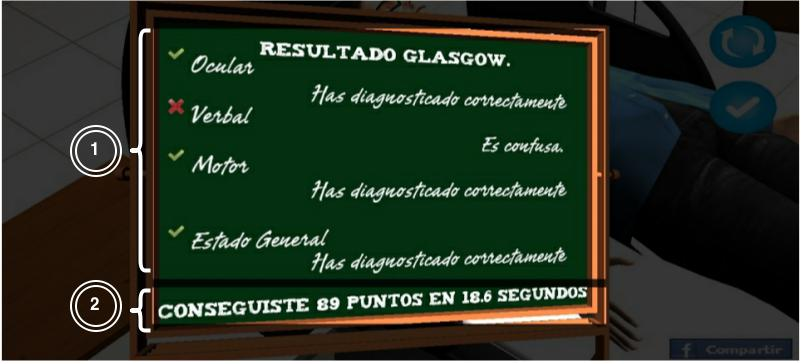
\includegraphics[width=10cm]{solucion/images/glasgow_resultado.jpg}
\caption{Retroalimentación y puntuación final del procedimiento de valoración de 
la escala de Glasgow.}
\label{fig:glasgow_resultado}
\end{figure}

\end{itemize}

\subsubsection{Registro de actividad}

Cada acción que realiza el usuario dentro de la simulación provoca un evento, y
estos eventos son registrados de manera transparente para el usuario. Como así 
también los eventos que genera la aplicación.

El registro de actividades permite reproducir las partidas y por lo tanto, es 
posible determinar que tareas fueron con las que los usuarios tuvieron un 
mayor número de inconvenientes.

%Tanto las acciones de los usuarios como otras informaciones incluyendo el diagnóstico 
%son almacenadas en un archivo en formato \Gls{json} y enviadas
%a un servidor que almacena la información acerca de todos los usuarios.

En la tabla \ref{tab:glasgow_registro} se pueden observan los eventos registrados.

%\fixme{Al igual que en la escena de \emph{Extracción de sangre}, las acciones
%    del usuario son registradas en un archivo con formato \Gls{json} y enviadas
%    a un servidor que almacena la información acerca de todos los usuarios.
%}{Concéntrense en lo que tienen que explicar sin comparar con otros casos por
%    que sino el párrafo se vuelve largo y pierde foco}

%Se almacena además, el diagnóstico del usuario, la puntuación del mismo y el
%estado inicial del paciente, así como el modo de la escena (evaluación o
%exploración).

\begin{table}[H]
\centering
\begin{tabulary}{\textwidth}{|L|L|L|}
\hline
Acción & Eventos & Motivos \\
\hline
Estímulos dolorosos & Estimulación de extremidades del paciente & Validación de la hipótesis 
\enquote{Acciones por menú} contextual \\
\hline
Acciones de voz  & Solicitudes y preguntas al paciente & Validación de la hipótesis \enquote{Comandos 
de voz} \\
\hline
Diagnóstico del paciente & Valoración del usuario acerca de la respuesta motora, verbal y ocular 
del paciente así como su estado general & Validación de interfaz intuitiva, de realización correcta de 
la valoración \\
\hline
Utilización de redes sociales & Socialización del resultado de la partida & Medición del efecto motivador\\
\hline
\end{tabulary}
\caption{Acciones registradas durante una partida del procedimiento de valoración de la ecala 
de Glasgow, los eventos relacionados a ellas, y los motivos de sus registros.}
\label{tab:glasgow_registro}
\end{table}


\subsubsection{Interfaz de usuario}

La interfaz de usuario, como se observa en la figura~\ref{fig:glasgow_gui}, es
muy sencilla, se compone de solo una opción permanente, la cual permite al
usuario finalizar la escena y mostrar la \emph{Pantalla de diagnóstico}. Se
observan además, las opciones que se despliegan cuando la solución detecta que el
usuario emite palabras, conocidas como \emph{Comandos de Voz}, que permiten al
mismo interactuar con el paciente.

\begin{figure}[H]
\centering
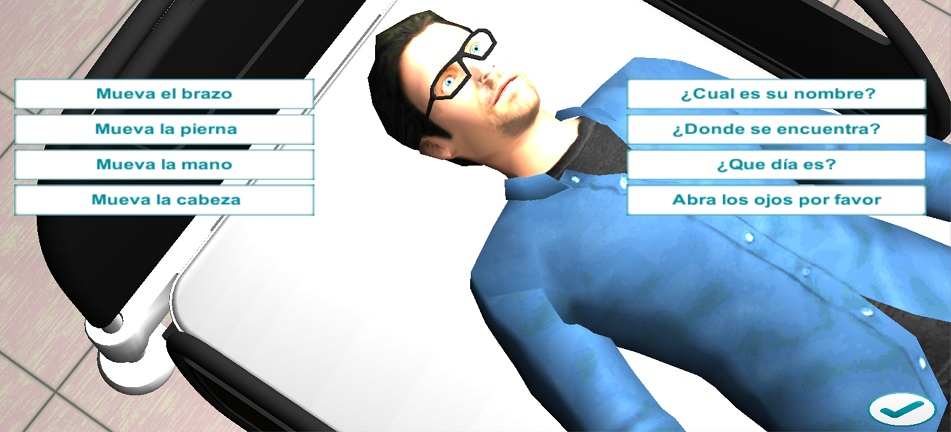
\includegraphics[scale=0.5]{solucion/images/glasgow_comandos_voz.jpg}
\caption{Interfaz de la escena \emph{Evaluación de Glasgow}, se observan los
    \emph{comandos de voz}, así como la opción que permite finalizar la escena
    (esquina inferior derecha).}
\label{fig:glasgow_gui}
\end{figure}

Además se ve en la interfaz, al paciente, que es el foco principal de la cámara.

\subsection{Pantalla de resultados}

Al finalizar ambas escenas, se presenta una pantalla de resultados, la cual es
la encargada de mostrar toda la información que fue recabada durante la escena,
esta información incluye los pasos correctos e incorrectos que realizó el
usuario.

\begin{figure}[H]
\centering
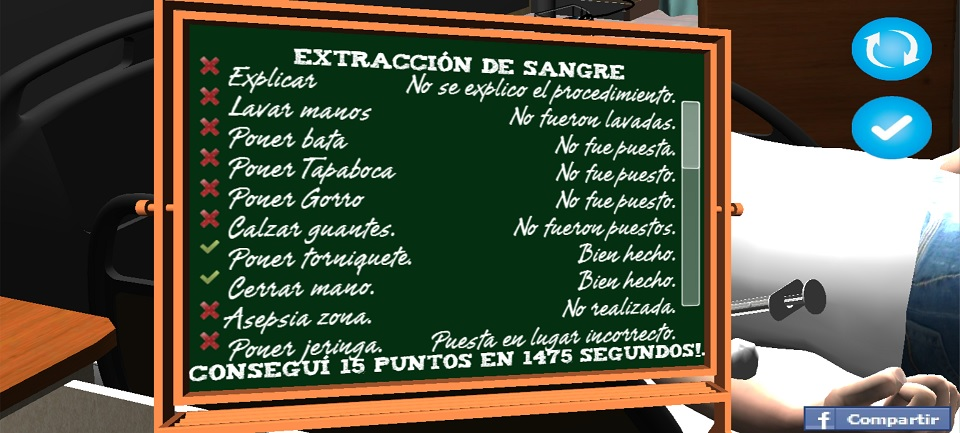
\includegraphics[scale=0.5]{solucion/images/resultado_hemocultivo.jpg}
\caption{Pantalla de resultados mostrando los pasos correctos e incorrectos, en
    la escena \emph{Glasgow}.}
\label{fig:resultados_glasgow}
\end{figure}

Se observa en la figura~\ref{fig:resultados_glasgow} el diseño de la
pantalla, el título es la escena actual, un resumen de la
puntuación, y el tiempo que duró la escena.

%Se lista de manera ordenada los pasos en la parte izquierda de la pantalla, y en
%la parte derecha se muestra información relevante acerca del motivo por el cual
%no se cumplió cada paso o es caso contrario, se indica que el pao fue realizado 
%correctamente.

Adicionalmente a la información de la sesión, se permite al usuario reiniciar la
partida, ir al menú, y compartir sus logros en las redes sociales.

Si el usuario presiona el botón \enquote{Facebook}, se despliega el menú de
dicha red social, permitiendo que el mismo pueda agregar un mensaje
personalizado y el resultado de la sesión se comparta con el texto \enquote{Conseguí 15 puntos
    en 1475 segundos, en la \emph{Escena Extracción de sangre} jugando con
    YAVE}.

